\documentclass{amsart}

\usepackage[utf8]{inputenc}
\usepackage[T2A]{fontenc}
\usepackage[english,russian]{babel}
\usepackage{amsthm,amsmath,amsfonts,amssymb}
\usepackage{fullpage}
\usepackage{eufrak}
\usepackage{bbm}
\usepackage { graphicx }

%%% Дополнительная работа с математикой
\usepackage{amsfonts,amssymb,amsthm,mathtools} % AMS
\usepackage{amsmath}
\usepackage{icomma}

%% Шрифты
\usepackage{euscript}	% Шрифт Евклид
\usepackage{mathrsfs}	% Красивый матшрифт

%% Свои команды
\DeclareMathOperator{\lb}{\mathop{lb}}	% логарифм по основанию 2
\DeclareMathOperator{\sgn}{\mathop{sgn}}	% сигнум
\renewcommand{\Im}{\mathop{\mathrm{Im}}\nolimits}	% мнимая часть
\renewcommand{\Re}{\mathop{\mathrm{Re}}\nolimits}	% вещественная часть
\renewcommand{\emptyset}{\varnothing}	% пустое множество
\renewcommand{\le}{\leqslant}	% отечественная версия "меньше или равно"
\renewcommand{\ge}{\geqslant}	% отечественная версия "больше или равно"
\renewcommand{\epsilon}{\varepsilon}	% стандартная "эпсилон"
\renewcommand{\phi}{\varphi}	% стандартная "фи"
\newcommand{\const}{\mathrm{const}}	% константа

%% Множества чисел
\DeclareMathOperator{\Natural}{\mathbb{N}}	% Натуральные числа
\DeclareMathOperator{\Integer}{\mathbb{Z}}	% Целые числа
\DeclareMathOperator{\Integerp}{\mathbb{Z}_{+}}	% Целые неотрицательные числа
\DeclareMathOperator{\Rational}{\mathbb{Q}}	% Рациональные числа
\DeclareMathOperator{\Real}{\mathbb{R}}	% Вещественные числа
\DeclareMathOperator{\Realp}{\mathbb{R}_{>0}}	% Вещественные положительные числа
\DeclareMathOperator{\Realn}{\mathbb{R}_{<0}}	% Вещественные отрицательные числа
\DeclareMathOperator{\Realnn}{\mathbb{R}_{\ge 0}}	% Вещественные неотрицательные числа
\DeclareMathOperator{\Realnp}{\mathbb{R}_{\le 0}}	% Вещественные неположительные числа
\DeclareMathOperator{\Complex}{\mathbb{C}}	% Комплексные числа

%% Заглавные греческие буквы
\DeclareMathOperator{\Alpha}{\mathrm{A}}	% Альфа
\DeclareMathOperator{\Beta}{\mathrm{B}}	% Вета
\DeclareMathOperator{\Epsilon}{\mathrm{E}}	% Эпсилон
\DeclareMathOperator{\Zeta}{\mathrm{Z}}	% Дзета
\DeclareMathOperator{\Eta}{\mathrm{H}}	% Эта
\DeclareMathOperator{\Iota}{\mathrm{I}}	% Йота
\DeclareMathOperator{\Kappa}{\mathrm{K}}	% Каппа
\DeclareMathOperator{\Mu}{\mathrm{M}}	% Мю
\DeclareMathOperator{\Nu}{\mathrm{N}}	% Ню
\DeclareMathOperator{\Omicron}{\mathrm{O}}	% Омикрон
\DeclareMathOperator{\Rho}{\mathrm{P}}	% Ро
\DeclareMathOperator{\Tau}{\mathrm{T}}	% Тау
\DeclareMathOperator{\Chi}{\mathrm{X}}	% Хи

%% Теория вероятностей
\renewcommand{\Prob}{\mathbb P}	% вероятность
\newcommand{\Expect}{\mathbb E}	% математическое ожидание
\renewcommand{\Variance}{\mathbb D}	% дисперсия
\newcommand{\Entropy}{\mathbb H}	% энтропия
\DeclareMathOperator{\cov}{\mathop{cov}}	% ковариация
\DeclareMathOperator{\supp}{\mathop{supp}}	% носитель
\DeclareMathOperator{\Skewness}{\mathop{Skew}}	% коэффициент асимметрии
\DeclareMathOperator{\Kurtosis}{\mathop{Kurt}}	% коэффициент эксцесса

%%% Статистический анализ
\newcommand*{\moment}[1]{\overline{#1}}	% выборочный момент
\DeclareMathOperator{\hskew}{\mathop{\widehat{Skew}}}	% выборочный коэффициент асимметрии
\DeclareMathOperator{\hkurt}{\mathop{\widehat{Kurt}}}	% выборочный коэффициент эксцесса
%% Однопараметрические распределения
\newcommand*{\chisq}[1]{\chi^2_{#1}}	% Распределение хи-квадрат
\newcommand*{\Stud}[1]{\mathcal{S}_{#1}}	% Распределение Стьюдента
\newcommand*{\Exp}[1]{\mathop{\mathrm{Exp}}(#1)}	% Показательное распределение
\newcommand*{\Bern}[1]{\mathop{\mathrm{Bern}}(#1)}	% Распределение Бернулли
\newcommand*{\Geom}[1]{\mathop{\mathrm{Geom}}(#1)}	% Геометрическое распределение
\newcommand*{\Pois}[1]{\mathop{\mathrm{Pois}}(#1)}	% Распределение Пуассона
%% Двухпараметрические распределения
\newcommand*{\FS}[2]{\mathcal{F}_{#1, #2}}	% Распределение Фишера-Снедекора
\newcommand*{\Norm}[2]{\mathcal{N}(#1, #2)}	% Нормальное распределение
\newcommand*{\Unif}[2]{\mathcal{U}(#1, #2)}	% Равномерное распределение
\newcommand*{\DE}[2]{\mathop{\mathrm{DE}}(#1, #2)}	% Распределение Лапласа
\newcommand*{\Cauchy}[2]{\mathop{\mathrm{C}}(#1, #2)}	% Распределение Коши
\newcommand*{\Binom}[2]{\mathop{\mathrm{Binom}}(#1, #2)}	% Биномиальное распределение
\newcommand*{\Betadist}[2]{\mathop{\mathrm{Beta}}(#1, #2)}	% Бета-распределение
\newcommand*{\Gammadist}[2]{\mathop{\mathrm{Gamma}}(#1, #2)}	% Гамма-распределение
%% Ажурные и готические буквы
\newcommand*{\Acl}{\mathcal{A}}	% A красивое
\newcommand*{\Ccl}{\mathcal{C}}	% C красивое
\newcommand*{\Fcl}{\mathcal{F}}	% F красивое
\newcommand*{\Icl}{\mathcal{I}}	% I красивое
\newcommand*{\Kcl}{\mathcal{K}}	% K красивое
\newcommand*{\Pcl}{\mathcal{P}}	% P красивое
\newcommand*{\Ycl}{\mathcal{Y}}	% Y красивое
\newcommand*{\Afr}{\mathfrak{A}}	% A готическое
\newcommand*{\Bfr}{\mathfrak{B}}	% B готическое
\newcommand*{\Ffr}{\mathfrak{F}}	% F готическое
\newcommand*{\Kfr}{\mathfrak{K}}	% K готическое
\newcommand*{\Xfr}{\mathfrak{X}}	% X готическое
%% Теория оценивания
\newcommand*{\ind}[1]{\mathbbm{1}_{\lbrace #1 \rbrace}}	% индикаторная функция
\newcommand*{\bias}[2]{\mathop{\mathrm{bias}}\nolimits_{#1}(#2)}	% смещение

%% Перенос знаков в формулах (по Львовскому)
\newcommand*{\hm}[1]{#1\nobreak\discretionary{}
	{\hbox{$\mathsurround=0pt #1$}}{}}

%%% Работа с картинками
\usepackage{graphicx,xcolor}	% Для вставки рисунков
\graphicspath{{images/}{images2/}}	% папки с картинками
\setlength\fboxsep{3pt}	% Отступ рамки \fbox{} от рисунка
\setlength\fboxrule{1pt}	% Толщина линий рамки \fbox{}
\usepackage{wrapfig}	% Обтекание рисунков и таблиц текстом
\RequirePackage{caption}
\DeclareCaptionLabelSeparator{defffis}{ "--- }
\captionsetup{justification=centering,labelsep=defffis}
\usepackage{float}
\usepackage{tikz}
\usepackage{pgfplots}
\pgfplotsset{compat=newest}
\usetikzlibrary{patterns}
\usetikzlibrary{calc}

%%% Работа с таблицами
\usepackage{array,tabularx,tabulary,booktabs}	% Дополнительная работа с таблицами
\usepackage{longtable}	% Длинные таблицы
\usepackage{multirow}	% Слияние строк в таблице
\usepackage{makecell}
\usepackage{multicol}


\renewcommand{\qedsymbol}{}

\newtheorem{problem}{Задание}

\begin{document}
	\newcommand{\problemset}[1]{
		\begin{center}
			\Large #1
		\end{center}
	}

	\begin{tabbing}
	\hspace{11cm} \= Студент: \= Майоров Артемий \\	% не забудьте исправить, студент Вы или студентка :)
																									% (а то некоторые забывают)
	\> Группа: \> 2375 \\	% Здесь меняете № группы
	\> Вариант: \> 14 \\		% А здесь меняете № варианта
	\> Дата: \> \today		% А вот здесь ничего не меняем!!!
\end{tabbing}
\hrule
\vspace{1cm}	% в данном файле меняем только Пол, Фамилию Имя, № группы и № варианта
	\problemset{Теория вероятностей и математическая статистика}
\problemset{Индивидуальное домашнее задание №1}	% поменяйте номер ИДЗ

\renewcommand*{\proofname}{Решение}

%%%%%%%%%%%%%% ЗАДАНИЕ №1 %%%%%%%%%%%%%%
%% Условие задания №1
\begin{problem}
        5 красных карточек и 7 синих карточек наудачу разложены по 4-м папкам. Найти вероятность того, что в каждой папке будут карточки двух цветов.
\end{problem}

%% Решение задания №1
\begin{proof}
    Пусть событие $A$ --- "В каждой папке карточки двух цветов". Разложим 5 красных карточек по 4-м папкам. ${{5 + 1 + (4 - 1) - 1} \choose {4 - 1}} = {8 \choose 3}$. Аналогично для синих карточек: ${{7 + 1 + (4 - 1) - 1} \choose {4 - 1}} = {10 \choose 3}$, следовательно общее число исходов будет равно: $\# \Omega = {8 \choose 3} \cdot {10 \choose 3} = 6720.$ Число благоприятных исходов будет считаться аналогично, только теперь нам необходимо, чтобы хотя бы 1 карточка была в папке. Для красных карточек: ${{5 - 1} \choose {4 - 1}} = {4 \choose 3}$, для синих: ${{7 - 1} \choose {4 - 1}} = {6 \choose 3}$, следовательно общее число благоприятных исходов будет равно: $\#A = {4 \choose 3} \cdot {6 \choose 3} = 80.$ Тогда по определению вероятности:\newline
    $\mathbb{P}A = \frac{\#A}{\#\Omega} = \frac{80}{6720} \approx 0,0119\newline$
    \newline
Ответ: 0,0119
\end{proof}

%%%%%%%%%%%%%% ЗАДАНИЕ №2 %%%%%%%%%%%%%%
%% Условие задания №2
\begin{problem}
	Прямые разбивают плоскость на полосы ширины 6. Определить вероятность того, что отрезок длины 2, наугад брошенный на плоскость, не пересечет ни одной прямой
\end{problem}

%% Решение задания №2
\begin{proof}
$\newline a = 3\newline r = 1\newline \mathbb{P}A$ --- вероятность, что отрезок не пересечет прямую. \newline $\mathbb{P}B$ --- вероятность, что отрезок пересечет прямую. \newline
\begin{figure}[H]
    \centering
    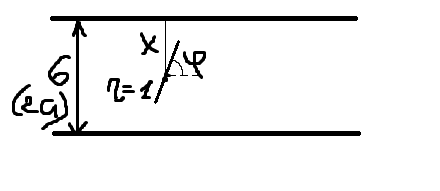
\includegraphics[width=0.5\linewidth]{1idz_1.png}
    \caption{Геометрическое представление задачи}
\end{figure}
	Возможные положения отрезка на плоскости полностью определяются положением центра отрезка и углом поворота отрезка относительно какого-либо направления – для удобства выберем в качестве направления прямую, параллельную исходным двум, и зададим положение отрезка углом между иголкой и этой прямой (он будет от 0 до $\pi$ обозначим его через $\phi$). Причём две эти переменные (положение центра и угол поворота) меняются независимо друг от друга. Обозначим через  расстояние от середины отрезка до ближайшей прямой, это расстояние находится в промежутке от 0 до $a$. Следовательно, можно посчитать меру всего пространства исходов. Это будет некий прямоугольник, одна сторона которого $\pi$, а другая $a$. Площадь этого прямоугольника:\newline
 $S = \pi \cdot a\newline$
 Посчитаем благоприятные исходы. Отрезок пересекает ближайшую прямую, если расстояние от середины отрезка до ближайшей прямой не превосходит $r \cdot \sin{\phi}\newline$
 Найдем площаль синусоиды $P$: \newline
 $P = \int_{0}^{\pi} r \cdot \sin{\phi} d \phi = 2 \cdot r\newline$
 \begin{figure}[H]
     \centering
     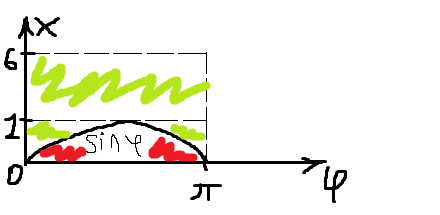
\includegraphics[width=0.5\linewidth]{1швя_2.png}
     \caption{График}
     \label{fig:enter-label}
 \end{figure}
 Для нахождения вероятность того, что отрезок пересечёт какую-нибудь прямую, необходимо разделить площадь синусоиды $P$ на площадь прямоуольника $S$:\newline
 $\mathbb{P}B = \frac{\#P}{\#S} = \frac{2 \cdot r}{a \cdot \pi} = \frac{2}{3 \cdot \pi}\newline$
 Вероятность того, что отрезок НЕ пересечет $\mathbb{P}A = 1 - \mathbb{P}B = 1 - \frac{2}{3 \cdot \pi} \approx 0,7878\newline$
 \newline
 Ответ: 0,7878
\end{proof}

%%%%%%%%%%%%%% ЗАДАНИЕ №3 %%%%%%%%%%%%%%
%% Условие задания №3
\begin{problem}
	В первой урне находится 8 белых и 8 черных шаров, во второй --- 8 белых и 18 черных шаров. Одновременно из первой и второй урн вытаскивают по шару, перемешивают и возвращают по одному в каждую урну. Затем из каждой урны вытаскивают по шару. Они оказались одного цвета. Определить вероятность того, что в первой урне осталось столько же белых шаров, сколько было вначале.
\end{problem}

%% Решение задания №3
\begin{proof}
	Определим полную группу событий:$\newline$
$H1$ --- "Из первого ящика достали белый и вернули белый"$\newline$
$H2$ --- "Из первого ящика достали белый и вернули черный"$\newline$
$H3$ --- "Из первого ящика достали черный и вернули белый"$\newline$
$H4$ --- "Из первого ящика достали черный и вернули черный"$\newline$
Событие $A$ --- "В первом ящике осталось столько же белых шаров".$\newline$
$\mathbb{P}(H1) = \frac{8}{16} \cdot \frac{8}{26} = \frac{2}{13} \newline$
$\mathbb{P}(H2) = \frac{8}{16} \cdot \frac{18}{26} = \frac{9}{26} \newline$
$\mathbb{P}(H3) = \frac{8}{16} \cdot \frac{8}{26} = \frac{2}{13} \newline$
$\mathbb{P}(H4) = \frac{8}{16} \cdot \frac{18}{26} = \frac{9}{26} \newline$

$\mathbb{P}(A|H1) = \frac{8}{16} \cdot \frac{18}{26} = \frac{9}{26}$ (чч) \newline
$\mathbb{P}(A|H2) = 0$ (т.к. в 1-ой урне недостаточно белых) \newline
$\mathbb{P}(A|H3) = \frac{9}{16} \cdot \frac{7}{26} = \frac{63}{416}$ (бб) \newline
$\mathbb{P}(A|H4) = \frac{8}{16} \cdot \frac{18}{26} = \frac{9}{26}$ (чч) \newline

\begin{center}
		\begin{tabular}{|c|c|c|c|c|c|}
			\hline
			$ Hi $  & $ H1 $ & $H2$ & $ H3 $ & $ H4 $ & $ \Sigma $ \\ \hline
			$ \mathbb{P}(Hi) $ & $\frac{2}{13}$ & $ \frac{9}{26}$ & $\frac{2}{13}$&$\frac{9}{26}$  & 1        \\ \hline
                $ \mathbb{P}(A|Hi) $ &$\frac{9}{26}$& 0&$\frac{63}{416}$&$\frac{9}{26}$& ---
                \\ \hline
		\end{tabular}
	\end{center}

 Найдем вероятность события $A$, используя формулу полной вероятности:\newline
 $\mathbb{P}(A) = \sum_{i=0}^4  \mathbb{P}(A|Hi) \cdot \mathbb{P}(Hi) = \frac{2}{13} \cdot \frac{9}{26} + 0 + \frac{2}{13} \cdot \frac{63}{416} + \frac{9}{26} \cdot \frac{9}{26} = \frac{531}{2704} \approx 0,1964\newline$

 Ответ: 0,1964

\end{proof}

%%%%%%%%%%%%%% ЗАДАНИЕ №4 %%%%%%%%%%%%%%
%% Условие задания №4
\begin{problem}
	При посылке сообщения, состоящего из 20-ти символов вероятность искажения каждого символа равна 0.01. Для надежности сообщение передается трижды. При этом известно, что при первой передаче были точно искжены первые 11 символов, а при последней передаче были искажены символы с 10-го по 20-й. Определить вероятность того, что на основании трех передач сообщение удастся восстановить.  
\end{problem}

%% Решение задания №4
\begin{proof}
	Обозначим события, вероятность которого требуется найти: 
 $A$ --– на основании трёх передач сообщение удастся восстановить.\newline
 $B$ --- есть неискаженный символ среди двух сообщений\newline
 $C$ --- получены символы 1--9\newline
 $D$ --- получены символы 10--11\newline
 $E$ --- получены символы 12--20\newline
 $p = 0,01$ --- вероятность искажения любого символа.\newline
 В событиях $C$ и $E$ в одном из сообщений символы искажены, поэтому там считаем вероятность из двух сообщений. В событии $D$ символы не искажены лишь в одном сообщении, поэтому там будем считать вероятность из одного сообщения:\newline
 $\mathbb{P}(B) = 1 - 0,01^2 = 0,9999\newline$
 $\mathbb{P}(C) =\mathbb{P}(B)^9 = 0,9991\newline$
 $\mathbb{P}(D) = (1 - 0,01)^2 = 0,9801\newline$
 $\mathbb{P}(E) = \mathbb{P}(B)^9 = 0,9991\newline$
 $\mathbb{P}(A) = \mathbb{P}(C) \cdot \mathbb{P}(D) \cdot \mathbb{P}(E) = 0,9783 \newline$
 \newline
 Ответ: 0,9783
\end{proof}

%%%%%%%%%%%%%% ЗАДАНИЕ №5 %%%%%%%%%%%%%%
%% Условие задания №5
\begin{problem}
	Вероятность успеха в схеме Бернулли равна $\frac{1}{4}$. Проводится 500 испытаний. Написать точную формулу и вычислить приближенную вероятность того, что число успехов попадет в интервал 115--135. 
\end{problem}

%% Решение задания №5
\begin{proof}
$\newline p = \frac{1}{4}\newline$
$n = 500\newline$
$np = 125 > 10$, следовательно будем использовать алгоритм Муавра-Лапласа. Сначала найдем общую формулу:\newline
1) $\mathbb{P}(A) = \sum_{m=115}^{135} {500 \choose m} \cdot \left(\frac{1}{4}\right)^m \cdot \left(\frac{3}{4}\right)^{500-m}\newline$
Теперь найдем вероятность:\newline
2) $\Phi(x2) - \Phi(x1) = \Phi(\frac{135 - 125}{\sqrt{125 \cdot 0,75}}) - \Phi(\frac{115 - 125}{\sqrt{125 \cdot 0,75}}) = \Phi(1,0328) \cdot 2 = 0,697\newline$
\newline
Ответ: 0,697

\end{proof}	% для удобства создаём по аналогии файлы ihw1.tex, ihw2.tex, etc
										% и просто меняем имя при компиляции
\end{document}